\chapter{A Potpourri of Proofs}

\begchap{I}n this chapter, we will walk through some more proofs which are comprehensive of the methods we previously discussed and are interesting results in of themselves. We will first discuss common traps to avoid. This end-of-book capstone chapter is not a comprehensive list of all the things we have learned, but rather, a set of a few theorems to which such methods can be applied. The proofs have been structured in a way so as to allow the flow of one statement directly from the previously proved statement, similar almost to a narrative arc. Each result has its own supporting theorems and statements, which culminate in the use in the proof of the main statement itself. 

\section{Common Traps}
There are many traps we must avoid in constructing a proof. One major trap is a circular argument. It essentially is saying that some thing is true because it is true. However, they may not always be so easily laid out. Consider the following example, taken from one of my favorite books, Art of Problem Solving Vol. 1: The Basics by Richard Rusczyk and Sandor Lehockzy. 
\begin{example}
Suppose 5 women and 5 men are seated at a round table such that each person sits between 2 people of the opposite gender. We shall prove that if we number the chairs from 1 to 10 in order, a woman must be seated in chair 1.
\end{example}
\begin{proof}
If a woman is in chair 1, a man must be in chair 2, so a woman must be in chair 3, a man in chair 4, a woman in chair 5, a man in chair 6, a woman in chair 7, a man in chair 8, a woman in chair 9, and a man in chair 10. Since chair 10 is next to chair 1, a woman must be in chair 1.
\end{proof}
This is a basic example of a circular argument (it need not involve a circle!). We attempt a direct proof, but our proof assumes that a woman is in chair 1, which is the very statement we wish to prove. If we wish to prove statement $X$, what we have shown above is $X \implies X$. This is also known as a tautology; something that is obviously true. It is always critical to avoid circular reasoning. It may often be helpful to make arrows between our statements, i.e. $A \implies B \implies C$ to map out our statements in a long and complex proof to avoid circular reasoning. We present a more complex example, one which is more subtle, in the appendix of this chapter. Be warned that this proof requires significant knowledge about derivatives and limits, concepts typically taught in a first-year calculus course.

We also need to be careful in checking the validity of our arguments, that the logic we use must be valid and mathematically correct. Consider the next example.
\begin{example}
$2 = 1$
\end{example}
\begin{proof}
Let $a, b \in \mathbb{R}$ such that $a = b$. Then,
\[
a^2 = ab
\]
\[
a^2-b^2 = ab-b^2
\]
\[
(a+b)(a-b) = b(a-b)
\]
\[
a+b = b
\]
And since $a = b$
\[
b + b = b
\]
\[
2b = b
\]
\[
2 = 1
\]
\end{proof}
Did you catch the mistake? I certainly did not! When I first heard of this in 6th grade, I spent nearly six months to disprove this and find the hole in the proof, though in retrospect, the hole in the proof is hidden in plain sight, so to speak.

\begin{exercise}
    Spend time  "debugging" the above proof. Why is it wrong?
\end{exercise}

One hint is that division by zero is illegal in math! 

The answer relies in the step in which we divided both sides by $a-b$. Since $a = b$, $a-b = 0$, and so we were dividing by zero! This illegal step led us to this unnatural answer, and once again is an exemplary proof of why we need to be careful in our proofs just as we would be careful in, say, arithmetic. If you want yet another example, and are familiar with calculus, consider the Chapter 5 Appendix. If not, feel free to skip it and return when you are familiar!

When considering your own proofs, be careful of these common logical traps! There are many more logical traps, but if you set out a clear if-then statement and a clear proof, then you will be able to catch some of these (most common) traps.

\section{Cyclic Quadrilaterals}
A cyclic quadrilateral is simply a quadrilateral in which all four points are concyclic - all four of its vertices lie on the same circle. Consider the following two quadrilaterals. 

\begin{center}
\begin{tikzpicture}[scale=1.2]

  % --- LEFT: cyclic quad ---
  \begin{scope}[xshift=-2.0cm]
    \draw[thick] (0,0) circle (1.4cm);
    
    \coordinate (A) at (100:1.4);
    \coordinate (B) at (20:1.4);
    \coordinate (C) at (310:1.4);
    \coordinate (D) at (210:1.4);

    \draw[thick] (A) -- (B) -- (C) -- (D) -- cycle;

    \filldraw[black] (A) circle (0.04) node[above]       {$A$};
    \filldraw[black] (B) circle (0.04) node[right]       {$B$};
    \filldraw[black] (C) circle (0.04) node[below right] {$C$};
    \filldraw[black] (D) circle (0.04) node[left]        {$D$};

    \node[font=\small] at (0, -1.9) {Cyclic quadrilateral};
  \end{scope}

  % --- RIGHT: non-cyclic quad (D lifted above circle) ---
  \begin{scope}[xshift=2.0cm]
    \draw[thick] (0,0) circle (1.4cm);

    \coordinate (A) at (100:1.4);
    \coordinate (B) at (20:1.4);
    \coordinate (C) at (310:1.4);
    % D is pulled inward/above the circle
    \coordinate (D) at ($(210:1.4) + (0.3, 2.3)$);

    \draw[thick] (A) -- (B) -- (C) -- (D) -- cycle;

    \filldraw[black] (A) circle (0.04) node[above]       {$A$};
    \filldraw[black] (B) circle (0.04) node[right]       {$B$};
    \filldraw[black] (C) circle (0.04) node[below right] {$C$};
    \filldraw[black] (D) circle (0.04) node[left]        {$D$};

    \node[font=\small] at (0, -1.9) {Non-cyclic quadrilateral};
  \end{scope}

\end{tikzpicture}
\end{center}

The quadrilateral on the left is a cyclic quadrilateral, while the quadrilateral on the right is not. This can bee seen visually since point D lies outside the circle on the right, but all four points lie on the circle on the left. 

Throughout this chapter, we will be proving various properties of cyclic quadrilaterals which are an invaluable subject of study, especially for competition math settings. It is not an overstatement that nearly half, if not more, of all geometry problems in high school mathematics competitions require the use of the properties of cyclic quadrilaterals - at least as an intermediate.

The fact that all four points lay on the same circle introduces very specific constraints on the angles (and consequently side lengths) of these quadrilaterals that we will attempt to prove throughout this section. Recall the inscribed angle theorem from chapter 3. This is a critical result we use in the proof of many following characteristic properties of cyclic quadrilaterals.

\begin{theorem}
$\angle AOB = 2 \angle ACB$.
\begin{center}
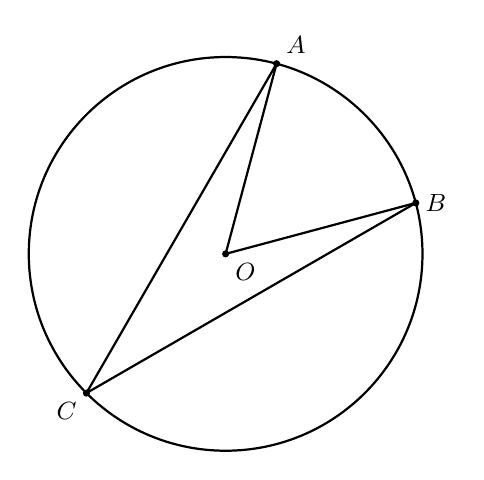
\begin{tikzpicture}[scale=2.5]

  % Circle
  \draw[thick] (0,0) circle (1);
  
  % Center
  \filldraw[black] (0,0) circle (0.015) node[below right, font=\small] {$O$};

  % Points A and B near each other (upper right area)
  \coordinate (A) at (75:1);
  \coordinate (B) at (15:1);
  
  % Point C opposite (lower left area)
  \coordinate (C) at (225:1);

  % Draw points
  \filldraw[black] (A) circle (0.015) node[above right, font=\small] {$A$};
  \filldraw[black] (B) circle (0.015) node[right, font=\small] {$B$};
  \filldraw[black] (C) circle (0.015) node[below left, font=\small] {$C$};

  % Lines CA and CB
  \draw[thick] (C) -- (A);
  \draw[thick] (C) -- (B);

  % Lines OA and OB (radii)
  \draw[thick] (0,0) -- (A);
  \draw[thick] (0,0) -- (B);
\end{tikzpicture}
\end{center}
\end{theorem}


We use this fact to prove the following important statement.

\begin{corollary}
The opposite angles of a cyclic quadrilateral sum to 180 degrees.
\end{corollary}

\begin{proof}
The proof is a simple application of the inscribed angle theorem (so much so that I have labeled this a corollary of the theorem rather than a standalone theorem). 
\begin{center}
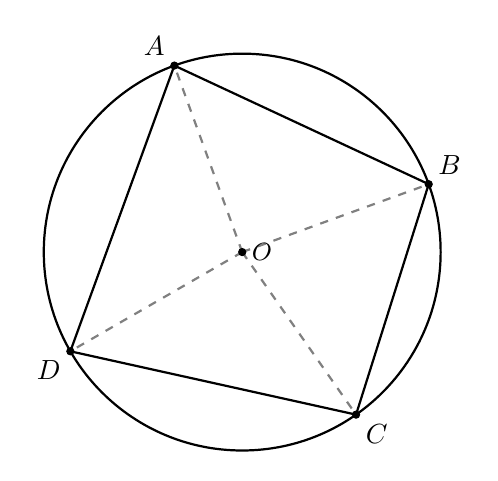
\begin{tikzpicture}[scale=1.8]

  \draw[thick] (0,0) circle (1.4cm);

  \coordinate (O) at (0,0);
  \coordinate (A) at (110:1.4);
  \coordinate (B) at (20:1.4);
  \coordinate (C) at (305:1.4);
  \coordinate (D) at (210:1.4);

  % Quadrilateral sides
  \draw[thick] (A) -- (B) -- (C) -- (D) -- cycle;

  % Lines from A and C to center
  \draw[thick, dashed, gray] (O) -- (A);
  \draw[thick, dashed, gray] (O) -- (B);
  \draw[thick, dashed, gray] (O) -- (C);
  \draw[thick, dashed, gray] (O) -- (D);

  % Points
  \filldraw[black] (A) circle (0.025) node[above left]  {$A$};
  \filldraw[black] (B) circle (0.025) node[above right] {$B$};
  \filldraw[black] (C) circle (0.025) node[below right] {$C$};
  \filldraw[black] (D) circle (0.025) node[below left]  {$D$};
  \filldraw[black] (O) circle (0.025) node[right, font=\small] {$O$};

\end{tikzpicture}
\end{center}
Consider the above diagram. We will first prove that the opposite angles $\angle BAD + \angle BCD = 180^{\circ}$. Via the inscribed angle theorem, we can get the following two relations
\[
2\angle BAD =  \angle BOD_1
\]
where angle $\angle BOD_1$ denotes the measure that is greater than $180^{\circ}$ (the side that opens upwards).
\[
2 \angle BCD = \angle BOD_2
\]
where angle $\angle BOD_1$ denotes the measure that is less than $180^{\circ}$ (the side that opens downwards). 

We also know that the sum of the central angles must be $360^{\circ}$. Therefore,
\[
\angle BOD_1 + \angle BOD_2 = 360^{\circ}
\]
and substituting with the relations derived from the inscribed angle theorem gives us
\[
2\angle BAD + 2\angle BCD = 360^\circ
\]
Dividing both sides by 2 gives us
\[
\angle BAD + \angle BCD = 180^{\circ}
\]
which has proved that opposite angles are supplementary (sum to $180^\circ$). A similar argument for $\angle ADB$ and $\angle ABC$ will give the same result (or the sum of all angles is $360^\circ$, so the other two angles must also sum to $180^\circ$). Thus, opposite angles sum to $180^\circ$ in a cyclic quadrilateral. 
\end{proof}

However, we can also proof the converse of this statement, that if opposite angles sum to $180^\circ$, then the quadrilateral is cyclic.

\begin{lemma}
If the opposite angles of a quadrilateral sum to $180^\circ$, then it is cyclic.
\end{lemma}
\begin{proof}
We will prove this via contradiction. Assume $ABCD$ is a non-cyclic quadrilateral that has opposite angles sum to $180^\circ$. First, WLOG, consider the three points $ABC$, which form a triangle. Then, consider the circumcircle of this triangle. 

\begin{center}
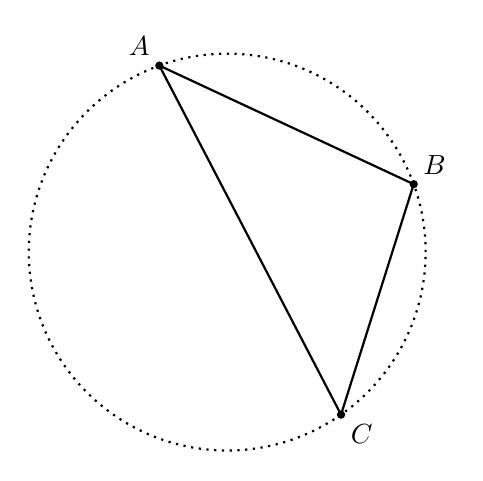
\begin{tikzpicture}[scale=1.8]

  \draw[dotted, thick] (0,0) circle (1.4cm);

  \coordinate (A) at (110:1.4);
  \coordinate (B) at (20:1.4);
  \coordinate (C) at (305:1.4);

  \draw[thick] (A) -- (B) -- (C) -- cycle;

  \filldraw[black] (A) circle (0.025) node[above left]  {$A$};
  \filldraw[black] (B) circle (0.025) node[above right] {$B$};
  \filldraw[black] (C) circle (0.025) node[below right] {$C$};

\end{tikzpicture}
\end{center}
Then, since the quadrilateral is not cyclic, the final point D must not be on the circle. WLOG, let lie outside of the circumcircle of $\triangle ABC$. Then, define D' as the intersection of ray $\vec{AD}$ with the circumcircle. Since the quadrilateral is not cyclic, we have that $D \neq D'$. 

\begin{center}
\begin{tikzpicture}[scale=1.8]

  \draw[dotted, thick] (0,0) circle (1.4cm);

  \coordinate (A) at (110:1.4);
  \coordinate (B) at (20:1.4);
  \coordinate (C) at (305:1.4);
  \coordinate (D') at (-1.35, -.376);
  \coordinate (D) at (210:1.9);

  % Ray from A through D' to D
  \draw[thick, gray, ->] (A) -- ($(A)!1.15!(D)$);

  % Triangle ABC (solid black)
  \draw[thick] (A) -- (B) -- (C) -- cycle;

  % Quadrilateral ABCD' (dashed blue)
  \draw[thick, dashed, blue!70!black] (A) -- (D') -- (C);

  % Quadrilateral ABCD (solid red)
  \draw[thick, red!70!black] (A) -- (D) -- (C);

  \filldraw[black] (A)  circle (0.025) node[above left]  {$A$};
  \filldraw[black] (B)  circle (0.025) node[above right] {$B$};
  \filldraw[black] (C)  circle (0.025) node[below right] {$C$};
  \filldraw[black] (D') circle (0.025) node[left, font=\small] {$D'$};
  \filldraw[black] (D)  circle (0.025) node[left]        {$D$};

\end{tikzpicture}
\end{center}
So the quadrilaterals $ABCD'$ and $ABCD$ may look something like the figure above. Since ABCD' is cyclic, we can derive some relations between the angles. First, we know that 
\[
\angle BAD' + \angle BCD' = 180^\circ
\]
Since $AD$ and $AD'$ lie on the same ray, we have that $\angle BAD' = \angle BAD$. Therefore, the equation becomes
\[
\angle BAD + \angle BCD' = 180^\circ
\]
However, we also know from the original condition of the statement that
\[
\angle BAD + \angle BCD = 180^\circ
\]
and therefore $\angle BCD' = \angle BCD$. But this is a contradiction. Considering the diagram, since $CD$ and $CD'$ are not on the same ray, the angles $\angle BCD$ and $\angle BCD'$ cannot be equal if $D \neq D'$. The only way $\angle BCD$ and $\angle BCD'$ can be equal is of $D = D'$, which is still a contradiction. 

Either way, we have now proved by contradiction that if opposite angles sum to $180^\circ$, quadrilateral $ABCD$ must be cyclic. 
\end{proof}

You may notice a potential error in the proof. It seems we used the original statement to prove the converse! We used the forwards direction, that if a quadrilateral is cyclic then its opposite angles must be supplementary to prove that if opposite angles are supplementary, the quadrilateral must be cyclic! However, there is a catch, and our use here is justified. 

The key distinction is specifically which quadrilateral we applied it to. If we applied the original statement to quadrilateral $ABCD$, then there would indeed be a logical error. It would be a circular statement! However, since we applied the theorem on quadrilateral $ABCD'$, which we already know to be cyclic (as opposed to quadrilateral $ABCD$, which we are trying to prove is cyclic), we can use the original statement. We are not doing a classic circular argument because we are not using the fact that 
\[
\text{$ABCD$ is cyclic} \implies \text{opposite angles are supplementary}
\]
to directly prove that 
\[
\text{opposite angles are supplementary}\implies \text{$ABCD$ is cyclic} 
\]
Instead, we know that $ABCD'$ is cyclic, which we use to prove that in $ABCD'$, opposite angles are supplementary, which is a perfectly fine, and an intended use of the statment. 

Furthermore, we have now proved the original statement both ways. We have constructed proofs of the statement
\[
\text{$ABCD$ is cyclic} \iff \text{opposite angles add to $180^\circ$}
\]

Now consider a similar, property of cyclic quadrilaterals which gives relationships between angles. 

\begin{theorem}
In cyclic quadrilateral $ABCD$, $\angle DAC = \angle DBC$, $\angle DCA = \angle DBA$, $\angle ACB = \angle ADB$, and $\angle BAC = \angle BDC$. 
\begin{center}
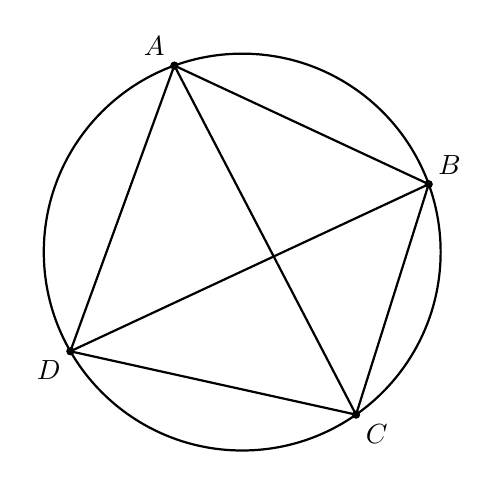
\begin{tikzpicture}[scale=1.8]

  \draw[thick] (0,0) circle (1.4cm);

  \coordinate (A) at (110:1.4);
  \coordinate (B) at (20:1.4);
  \coordinate (C) at (305:1.4);
  \coordinate (D) at (210:1.4);

  % Sides
  \draw[thick] (A) -- (B) -- (C) -- (D) -- cycle;

  % Diagonals
  \draw[thick, solid, black] (A) -- (C);
  \draw[thick, solid, black] (B) -- (D);

  \filldraw[black] (A) circle (0.025) node[above left]  {$A$};
  \filldraw[black] (B) circle (0.025) node[above right] {$B$};
  \filldraw[black] (C) circle (0.025) node[below right] {$C$};
  \filldraw[black] (D) circle (0.025) node[below left]  {$D$};

\end{tikzpicture}
\end{center}
\end{theorem}
\begin{proof}
We will prove that $\angle DAC = \angle DBC$. The remaining equalities are proven using the same logic and same approach.

Consider the angle $DOC$, where $O$ is the center of the circle. 

\begin{center}
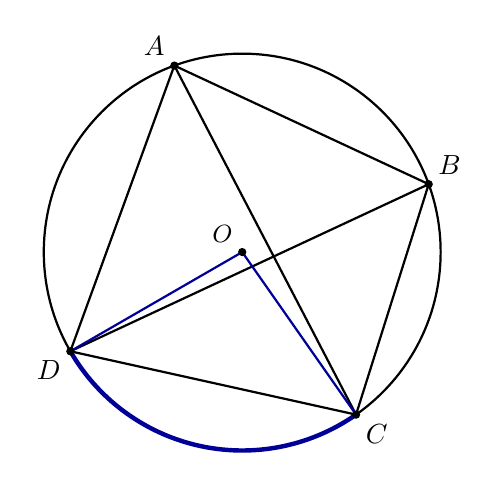
\begin{tikzpicture}[scale=1.8]
  \draw[thick] (0,0) circle (1.4cm);

  \coordinate (O) at (0,0);
  \coordinate (A) at (110:1.4);
  \coordinate (B) at (20:1.4);
  \coordinate (C) at (305:1.4);
  \coordinate (D) at (210:1.4);

  % Sides
  \draw[thick] (A) -- (B) -- (C) -- (D) -- cycle;

  % Diagonals
  \draw[thick, solid, black] (A) -- (C);
  \draw[thick, solid, black] (B) -- (D);

  % Lines OC and OD
  \draw[thick, blue!60!black] (O) -- (C);
  \draw[thick, blue!60!black] (O) -- (D);

  % Arc CD highlighted
  \draw[ultra thick, blue!60!black] (210:1.4) arc[start angle=210,
        end angle=305, radius=1.4cm];

  \filldraw[black] (A) circle (0.025) node[above left]  {$A$};
  \filldraw[black] (B) circle (0.025) node[above right] {$B$};
  \filldraw[black] (C) circle (0.025) node[below right] {$C$};
  \filldraw[black] (D) circle (0.025) node[below left]  {$D$};
  \filldraw[black] (O) circle (0.025) node[above left, font=\small] {$O$};

\end{tikzpicture}
\end{center}

Since the inscribed angle $\angle DAC$ subtends minor arc $AB$ (outlined in blue), and the central angle $\angle DOC$ subtends the same minor arc $AB$, we have that 
\[
\angle DOC = 2 \angle DAC
\]
Similarly, since the inscribed $\angle DBC$ subtends minor arc $AB$, and the central angle $\angle DOC$ subtends the same minor arc $AB$, we also have that
\[
\angle DOC = 2\angle DBC
\]
And by the transitive property
\[
2 \angle DAC = 2\angle DBC
\]
and therefore
\[
\angle DAC = \angle DBC
\]
By the exact same logic, we can construct a central angle for an arc subtended by two of the same inscribed angles in the cyclic quadrilateral and use it to prove that both inscribed angles that subtend the same arc have the same measure.
\end{proof}

The transitive property has been something we have so far not yet discussed. However, you know what this is already! Given two statements $A = B$ and $B = C$, the transitive property simply asserts that $A = C$. In our example,. we had that $2\angle DBC = \angle DOC$ and $\angle DOC = 2\angle DBC$, which gave us the answer that $2 \angle DAC = 2\angle DBC$.

As a side-note, this can also be applied to statements. For example, if 
\[
A \implies B ~~\text{    and    }~~ B \implies C
\]
then 
\[
A \implies C
\]
You may see the transitive property used in many other contexts as well, not restricted to equalities or if-then statements. However, it is usually obvious to understand where it is used, even if not cited; hence the name "property" and not something larger like "theorem" or "lemma". It is simply a property of the system of logic we use.

We will now prove the converse of the statement, with the end goal of proving the bidirectional statement.

\begin{theorem}
If $\angle DAC = \angle DBC$ (or any two such angles), then $ABCD$ is cyclic.
\end{theorem}
\begin{proof}
We will assume that $\angle DAC = \angle DBC$, but the proof will apply for any two such angles in a cyclic quadrilateral (see the proof above for the possible pairs). We will proceed via contradiction. Assume for contradiction that $\angle DAC = \angle DBC$ but $ABCD$ is not cyclic. As before, draw the circumcircle of $A$, $B$, $C$, and let $D'$ be the second intersection of ray $BD$ with the circumcircle, so that $D' \neq D$.
\begin{center}
\begin{tikzpicture}[scale=1.8]
  \draw[dotted, thick] (0,0) circle (1.4cm);

  \coordinate (A) at (110:1.4);
  \coordinate (B) at (20:1.4);
  \coordinate (C) at (305:1.4);
  \coordinate (D') at (210:1.4);
  \coordinate (D) at (210:1.9);

  % Ray from B through D' to D
  \draw[thick, gray, ->] (B) -- ($(B)!1.08!(D)$);

  % Triangle ABC
  \draw[thick] (A) -- (B) -- (C) -- cycle;

  % Diagonals
  \draw[thick, dashed, gray] (A) -- (C);

  % ABCD' in blue dashed
  \draw[thick, dashed, blue!70!black] (A) -- (D') -- (C);

  % ABCD in red solid
  \draw[thick, red!70!black] (A) -- (D) -- (C);

  \filldraw[black] (A)  circle (0.025) node[above left]  {$A$};
  \filldraw[black] (B)  circle (0.025) node[above right] {$B$};
  \filldraw[black] (C)  circle (0.025) node[below right] {$C$};
  \filldraw[black] (D') circle (0.025) node[left, font=\small] {$D'$};
  \filldraw[black] (D)  circle (0.025) node[left]        {$D$};
\end{tikzpicture}
\end{center}
Since $ABCD'$ is cyclic by construction, we apply the forward direction of the theorem
\[
\angle D'AC = \angle D'BC
\]
Now, $\angle D'BC = \angle DBC$ since $D'$ and $D$ both lie on ray $BD$, so the ray $BD'$ and ray $BD$ are the same ray. Therefore
\[
\angle D'AC = \angle DBC
\]
But by assumption, $\angle DAC = \angle DBC$. Therefore
\[
\angle D'AC = \angle DAC
\]
This means $D$ and $D'$ subtend the same angle at $A$ with respect to $AC$. Since $D$ and $D'$ both lie on the same ray from $B$, this forces $D = D'$. But $D'$ lies on the circumcircle and $D$ does not, which is a contradiction. Therefore $ABCD$ must be cyclic. (or D = D', either way works).
\end{proof}

You may notice a commonality between the proofs of the converses. We constructed a quadrilateral which we aimed to prove is cyclic $ABCD$. However, to do so, we constructed a second quadrilateral which we know is cyclic and used the assumption to prove that both quadrilaterals must be the same. This method, more generally, is sometimes known as the ghost point method. We construct a ghost point ($D'$) and argue directly that $D = D'$, which gives us the proof we need (or we use contradiction which could give a broader result). You may see it denoted by other names in other places, but by the construction of some "ghost point" and argument that a point must be equal to the ghost points is a powerful technique in olympiad geometry proofs. There are many more applications of this technique in olympiad geometry, so see the resources appendix for a recommendation to learn more!

Furthermore, with the conclusion of this proof, we have now proved the bidirectional statement that: $ABCD$ is cyclic if and only if angles with the same endpoints have the same measure
($D$ and $C$ in this case that we proved). However, note also the first bidirectional statement we proved
\[
\text{$ABCD$ is cyclic} \iff \text{opposite angles add to $180^\circ$}
\]
Thus, by the transitive property we can also find that: angles with the same endpoints have the same measure if and only if opposite angles add to $180^\circ$. We can therefore sum up our findings in a single theorem statement, which is how you will most commonly see these concepts be presented.
\begin{theorem}
The following statements are equivalent:
\begin{enumerate}
    \item $ABCD$ (or the quadrilateral in question) is cyclic
    \item opposite angles sum to $180^\circ$
    \item angles with the same endpoints have the same measure
\end{enumerate}
\end{theorem}

This means that if any one of the above is true, all three statements are true. If any one of the above statements is false, then all three of the above statements are false. In this way, we have a closely-knit web of statements that all mean the same thing, technically. If we know that opposite angles sum to $180^\circ$, then we know $ABCD$ (or the quadrilateral in question) is cyclic, and angles in the quadrilateral with the same endpoints have the same measure. In a similar fashion, if any one of the above statements is false, it implies that the other two are also false. This theorem is specifically why cyclic quadrilaterals are a powerful and very often used concept in olympiad geometry. 

Now consider the following result of cyclic quadrilaterals, which we will subsequently aim to prove.
\begin{theorem}[Ptolemy's Theorem]
Let $ABCD$ be a cyclic quadrilateral with sides $AB$, $BC$, $CD$, $DA$ 
and diagonals $AC$ and $BD$.
\begin{center}
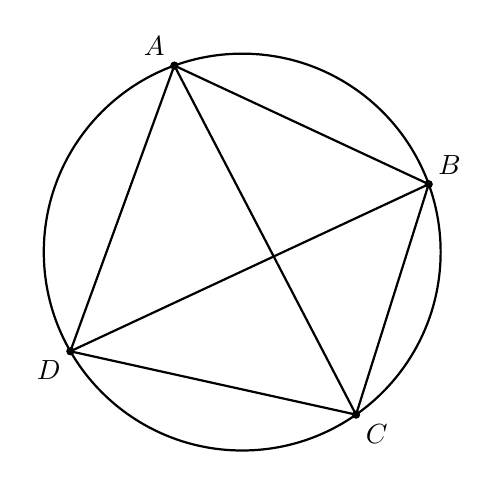
\begin{tikzpicture}[scale=1.8]
  \draw[thick] (0,0) circle (1.4cm);

  \coordinate (A) at (110:1.4);
  \coordinate (B) at (20:1.4);
  \coordinate (C) at (305:1.4);
  \coordinate (D) at (210:1.4);

  % Sides
  \draw[thick] (A) -- (B) -- (C) -- (D) -- cycle;

  % Diagonals
  \draw[thick, black] (A) -- (C);
  \draw[thick, black] (B) -- (D);

  \filldraw[black] (A) circle (0.025) node[above left]  {$A$};
  \filldraw[black] (B) circle (0.025) node[above right] {$B$};
  \filldraw[black] (C) circle (0.025) node[below right] {$C$};
  \filldraw[black] (D) circle (0.025) node[below left]  {$D$};

\end{tikzpicture}
\end{center}
Then 
\[
AC \cdot BD = AB \cdot CD + AD \cdot BC
\]
\end{theorem}

Before we begin the proof, we will consider a short detour as a primer of the concept of similar triangles, which we use in the proof itself. Similar triangles are two (or more) triangles which are the same up to some dilation, translation, and/or rotation. If it is possible to construct $\triangle ABC$ by dilating, translating, and/or rotating $\triangle DEF$, then we say the two triangles are similar
\[
\triangle ABC \sim \triangle DEF
\]
For example, consider the following figure.
\begin{center}
\begin{tikzpicture}[scale=1.3]

  % --- Similar pair (top) ---
  \begin{scope}[yshift=2.8cm]
    % Triangle 1
    \coordinate (A1) at (0, 0);
    \coordinate (B1) at (2.2, 0);
    \coordinate (C1) at (1.6, 1.1);

    \draw[thick, blue!70!black] (A1) -- (B1) -- (C1) -- cycle;

    \filldraw[black] (A1) circle (0.03) node[below left,  font=\small] {$A$};
    \filldraw[black] (B1) circle (0.03) node[below right, font=\small] {$B$};
    \filldraw[black] (C1) circle (0.03) node[above,       font=\small] {$C$};

    % Triangle 2 — scaled by 0.7 and rotated 100 degrees
    \coordinate (D1) at (4.8, 0);
    \coordinate (E1) at ($(D1) + ({0.7*2.2*cos(100)}, {0.7*2.2*sin(100)})$);
    \coordinate (F1) at ($(D1) + ({0.7*1.6*cos(145)}, {0.7*1.1*sin(145)})$);

    \draw[thick, red!70!black] (D1) -- (E1) -- (F1) -- cycle;

    \filldraw[black] (D1) circle (0.03) node[right,        font=\small] {$D$};
    \filldraw[black] (E1) circle (0.03) node[above,       font=\small] {$E$};
    \filldraw[black] (F1) circle (0.03) node[below left, font=\small] {$F$};

    \node[font=\small] at (2.8, -0.5) {$\triangle ABC \sim \triangle DEF$};
  \end{scope}

  % --- Not similar pair (bottom) ---
  \begin{scope}[yshift=-0.5cm]
    % Triangle 1 — tall and thin
    \coordinate (A2) at (0, 0);
    \coordinate (B2) at (1.8, 0);
    \coordinate (C2) at (0.3, 1.6);

    \draw[thick, blue!70!black] (A2) -- (B2) -- (C2) -- cycle;

    \filldraw[black] (A2) circle (0.03) node[below left,  font=\small] {$A$};
    \filldraw[black] (B2) circle (0.03) node[below right, font=\small] {$B$};
    \filldraw[black] (C2) circle (0.03) node[above,       font=\small] {$C$};

    % Triangle 2 — wide and flat
    \coordinate (D2) at (2.8, 0.4);
    \coordinate (E2) at (5.2, 0.4);
    \coordinate (F2) at (5.0, 1.3);

    \draw[thick, red!70!black] (D2) -- (E2) -- (F2) -- cycle;

    \filldraw[black] (D2) circle (0.03) node[below left,  font=\small] {$D$};
    \filldraw[black] (E2) circle (0.03) node[below,       font=\small] {$E$};
    \filldraw[black] (F2) circle (0.03) node[above right, font=\small] {$F$};

    \node[font=\small] at (2.8, -0.5) {$\triangle ABC \not\sim \triangle DEF$};
  \end{scope}

\end{tikzpicture}
\end{center}

In the first pair, triangles $\triangle ABC$ and $\triangle DEF$ are similar. This is because we can construct either triangle from a combination of dilations, rotations, and reflections without changing the underlying shape of the triangle. However, in the bottom pair, the triangles are not similar because their underlying shape itself is different and no combinations of the aforementioned transformations can map one triangle to the other; we would need to change the shape of the underlying triangle to be able to do so. 

One way of proving similarity is via the angles. Specifically, if two corresponding angles are the same, then the triangles are similar. This is called AA similarity (angle-angle similarity). The proof of this, while we won't formally prove it, hinges on the fact that if two angles of a triangle are the same, then since the sum of the angles is always $180^\circ$, then the third angle must be the same. Then, all three angles being the same necessitates that the relative structures of the figures must be the same (try constructing triangles with the same angles that are not similar). 

We can also derive relations among side lengths in similar triangles. Since the dilation factor must be the same across all axes (or else we would stretch and warp the triangle, which does not preserve its shape), we can relate the ratios between the sides. For example, in the first pair of triangles, we can get the relation
\[
\frac{AB}{DE} = \frac{BC}{EF} =\frac{AC}{DF}=\alpha
\]
for some $\alpha$ which is the dilation factor. This number is usually not of much interest, but if given, it can be very useful. As with all other concepts we have discussed, similar triangles is an especially important concept in olympiad geometry. While there are other ways to prove similarity and other theorems to do with similar triangles, this short primer provides enough background to begin our proof of Ptolemy's Theorem. 
\begin{proof}
Pick a point $E$ on BD such that $\angle DAE = \angle CAB$. 
\begin{center}
\begin{tikzpicture}[scale=1.8]
  \draw[thick] (0,0) circle (1.4cm);
  \coordinate (A) at (110:1.4);
  \coordinate (B) at (20:1.4);
  \coordinate (C) at (305:1.4);
  \coordinate (D) at (210:1.4);

  % E on BD — adjust t to slide E along BD
  \coordinate (E) at ($(B)!0.6!(D)$);

  % Sides
  \draw[thick] (A) -- (B) -- (C) -- (D) -- cycle;

  % Diagonals
  \draw[thick, black] (A) -- (C);
  \draw[thick, black] (B) -- (D);

  % Line AE
  \draw[thick, red!70!black] (A) -- (E);

  \filldraw[black] (A) circle (0.025) node[above left]  {$A$};
  \filldraw[black] (B) circle (0.025) node[above right] {$B$};
  \filldraw[black] (C) circle (0.025) node[below right] {$C$};
  \filldraw[black] (D) circle (0.025) node[below left]  {$D$};
  \filldraw[red!70!black] (E) circle (0.025) node[below right, font=\small] {$E$};
\end{tikzpicture}
\end{center}

Then, consider $\triangle DAE$ and $\triangle CAB$. We have that $\angle DAE = \angle CAB$ by construction, and $\angle ADB = \angle ACB$ by the property of inscribed angles in a cyclic quadrilateral. Therefore, since both these angles are the same in corresponding parts of the triangles, we conclude via AA similarity that 
\[
\triangle DAE \sim \triangle CAB
\]
From this similarity, we can get the relation that
\begin{equation}
\frac{BC}{AC} = \frac{ED}{AD}
\end{equation}
Next, we have that
\[
\angle BAE = \angle BAD - \angle DAE
\]
and since $\angle DAE = \angle CAB$
\[
\angle BAE = \angle BAD - \angle CAB
\]
which we can see via the figure is, by construction, 
\[
\angle BAE = \angle DAC
\]
Since by the properties of inscribed angles in cyclic quadrilaterals we can find that $\angle ABE = \angle ACD$, we can get another similarity relation
\[
\triangle ABE \sim \triangle ACD
\]
and from this relation we get that
\begin{equation}
\frac{AB}{BE} = \frac{AC}{CD}
\end{equation}
Cross-multiplying and rearranging both equation (5.1) and (5.2), we get the following set of equations
\[
\begin{cases}
BC \cdot AD = AC \cdot ED \\
AB \cdot CD = AC\cdot BE
\end{cases}
\]
We now add the two equations above
\[
AB\cdot CD + BC\cdot AD = AC\cdot ED + AC\cdot BE
\]
and factor the right-hand side
\[
AB\cdot CD + BC\cdot AD = AC \cdot (BE + ED)
\]
and since $BE + ED = BD$, we get the final statement
\[
AB\cdot CD + BC\cdot AD = AC \cdot BD
\]
which is exactly Ptolemy's Theorem.
\end{proof}

We have now proved a perhaps surprising yet useful result in geometry. This is widely used across Euclidean Geometry. We will see one such example of its use.

\begin{example}
Prove the Pythagorean Theorem using Ptolemy's Theorem.
\end{example}
\begin{proof}
We need two legs that meet at a right angle. Therefore, consider a rectangle inscribed in a circle. All rectangles are cyclic quadrilaterals, since opposite angles are both $90^\circ$ which always sum to $180^\circ$. 
\begin{center}
\begin{tikzpicture}[scale=1.8]

  \draw[thick] (0,0) circle (1.4cm);

  % Rectangle vertices — opposite vertices are diametrically opposite
  \coordinate (A) at (130:1.4);
  \coordinate (B) at (50:1.4);
  \coordinate (C) at (310:1.4);
  \coordinate (D) at (230:1.4);

  % Sides
  \draw[thick] (A) -- (B) -- (C) -- (D) -- cycle;

  % Diagonals
  \draw[thick, black] (A) -- (C);
  \draw[thick, black] (B) -- (D);

  \filldraw[black] (A) circle (0.025) node[above left]  {$A$};
  \filldraw[black] (B) circle (0.025) node[above right] {$B$};
  \filldraw[black] (C) circle (0.025) node[below right] {$C$};
  \filldraw[black] (D) circle (0.025) node[below left]  {$D$};

  % Side labels
  \node[font=\small] at ($(A)!0.5!(B) + (0.0, 0.15)$)  {$a$};
  \node[font=\small] at ($(B)!0.5!(C) + (0.15, 0.0)$)  {$b$};
  \node[font=\small] at ($(C)!0.5!(D) + (0.0, -0.15)$) {$a$};
  \node[font=\small] at ($(D)!0.5!(A) + (-0.15, 0.0)$) {$b$};

  % Diagonal label
  \node[black, font=\small] at ($(A)!0.5!(C) + (0.18, 0.1)$) {$c$};

  % Right angle marks at each corner
  \foreach \p/\a/\b in {A/B/D, B/C/A, C/D/B, D/A/C}{
    \path (\p) -- ++($0.12*(\a)-0.12*(\p)$) coordinate (t1);
    \path (\p) -- ++($0.12*(\b)-0.12*(\p)$) coordinate (t2);
    \path (t1) -- ++($(t2)-(\p)$) coordinate (t3);
    \draw[thin] (t1) -- (t3) -- (t2);
  }

\end{tikzpicture}
\end{center}
Consider the above inscribed rectangle, with opposite sides $AB = CD = a$ and $AD = BC = b$. The diagonals are equal (by definition of a rectangle) and thus let $AC = BD = c$. 

Ptolemy's theorem on this figure gives us 
\[
AB \cdot CD + AD \cdot BC = AC \cdot BD
\]
which simplifies to 
\[
a^2 + b^2 = c^2
\]
which is exactly the Pythagorean Theorem for right triangles $\triangle ACD, $ $\triangle ABC,$ $ \triangle DAB, $ and $\triangle DCB$. 
\end{proof}
The Pythagorean Theorem is nothing more than a special case of Ptolemy's Theorem applied to a rectangle! This is the second out of over 370 proofs of the Pythagorean Theorem. Hopefully you can begin to see why there are so many!

Ptolemy's theorem and the concepts of cyclic quadrilaterals are widely used across many domains. Keep these results in mind for the next time you encounter a quadrilateral - it may be cyclic!

\section{Wilson's Theorem}
Wilson's theorem is a result in number theory that is perhaps rarely used in competition mathematics. However, when it does get used, it is often very useful and and revolutionizes the solution. 

\begin{theorem}[Wilson's Theorem]
A positive integer $p$ is prime if and only if $(p-1)! \equiv -1 ~~ (\text{mod }p )$, where $x! = x \cdot (x-1) \cdots 2 \cdot 1$ is the factorial. 
\end{theorem}

Just take a moment to understand what this means. We will make a list below, showing heuristic evidence that this is true for somewhat small numbers. 

\begin{table}[h]
\centering
\begin{tabular}{|c|c|c|}
\hline
$p$ & $(p-1)!$ & $(p-1)! \pmod p$ \\ \hline
2 & 1 & 1 \\ \hline
3 & 2 & 2 \\ \hline
4 & 6 & 2 \\ \hline
5 & 24 & 4 \\ \hline
6 & 120 & 0 \\ \hline
7 & 720 & 6 \\ \hline
8 & 5,040 & 0 \\ \hline
9 & 40,320 & 0 \\ \hline
10 & 362,880 & 0 \\ \hline
11 & 3,628,800 & 10 \\ \hline
12 & 39,916,800 & 0 \\ \hline
13 & 479,001,600 & 12 \\ \hline
\end{tabular}
\caption{Wilson's Theorem verification for $2 \le p \le 13$}
\end{table}


We can see that Wilson's theorem does hold, that for prime numbers, the residue modulo $p$ is exactly $p-1$. This raises some questions we will try to address in this section. Try to think of what questions you have and how you may answer them as well as we explore deeper the mathematics behind Wilson's theorem. 

Before we begin any proof, we will first discuss modular residues for those not very familiar with it (we have thus far assumed you know what a mod is, but perhaps not the full system of modular arithmetic). 

The set of residues modulo $a$ is the set
\[
\{0, 1, \ldots, a-1 \}
\]
which is simply the set of all possible remainders when any number is divided by $a$. We know how to find a residue modulo $a$ because we know how to simply divide and find the remainder. However, operations in modular arithmetic are of special importance to us. 

First, it should be said that the set $\mathbb{Z}_{p}$ is a field for every prime $p$. You will encounter more on fields during study of abstract algebra, but for now, let us consider just the basics we need for the purpose of this book. 

A field is a set equipped with two operations, commonly denoted $+$ and $\times$ and called addition and multiplication, respectively. For our purposes, these symbols represent the numerical operation of addition of numbers and multiplication of numbers\footnote{I know this sounds overtly formal and redundant. However, abstract algebra is, as you guessed, quite abstract. Mathematicians have generalized these concepts to situations in which the operations of a field are not necessarily numerical addition or multiplication, but other operations that behave similarly! If you want to learn more, consider searching up "Rubiks cube group", which will show how operations in abstract algebra are not necessarily the ones we know best. Now, this is a group, which is another concept in abstract algebra, but will demonstrate the generality of abstract algebra and hopefully justify my word choice to you!}. A field must have certain properties, including that each operation has a unique identity element (i.e. $1$ for $\times$ and $0$ for $+$), every element has both an additive and multiplicative inverse (the additive identity need not have a multiplicative inverse), and the distributive property holds. We will not explore all of these conditions, but one specific condition is very useful in our proof of Wilson's theorem. 

Consider, for example, the field $\mathbb{Z}_7$. First, the operations themselves. The elements of this field are $\{0, 1, 2, 3, 4, 5, 6\}$. We can add residues (which is another name for elements in modular arithmetic, and these fields that embody modular arithmetic) using simple addition, for example
\[
3 + 4 \equiv 7 \equiv 0 ~ (\text{mod }7)
\]
As such, 3 and 4 are additive inverses in the field, since they add to the additive identity 0 ($x + 0 = x$; when the number stays the same after the operation, the 0 in this example is called the identity of the operation). Similarly, 2 and 5 are additive inverses as well. Furthermore, note that we can use negative numbers as well. For example
\[
4 \equiv -3 ~ (\text{mod }7)
\]
which makes it clear that it is the additive inverse of $3$.

Furthermore, we can look at multiplicative inverses as well. First, we identify the multiplicative identity, which we all know is 1. This is because $1 \times a = a$ for any $a \neq 0$ (the additive identity). Then, we are tasked with finding the multiplicative inverse element, which we typically denote $a^{-1}$ such that 
\[
a^{-1} \times a \equiv 1 ~ (\text{mod }7)
\]
Each element (other than zero) has a unique inverse if and only if  $p$ is prime, which we aim to compute. Since we are working with a small field (there are only 5 numbers to deal with), the best way of finding multiplicative inverses are by brute force. We will consider an example, to find the multiplicative inverse of $3$ in this field.

\begin{example}
    Find the multiplicative inverse of $3$ in $\mathbb{Z}_7$
\end{example}
\begin{proof}
    We are looking for the integer $b \in \{0, 1, 2, 3, 4, 5, 6\}$ such that 
    \[
    3 \times b \equiv 1~ (\text{mod }7)
    \]
    We will just go by brute force, skipping 0 and 1 (0 has no multiplicative inverse, and 1 is its own multiplicative inverse). 
    \[
    3 \times 2 \equiv 6 ~ (\text{mod }7)
    \]
    \[
    3 \times 3 \equiv 9 \equiv 2 ~ (\text{mod }7)
    \]
    \[
    3 \times 4 \equiv 12 \equiv 5 ~ (\text{mod }7)
    \]
    \[
    3 \times 5 \equiv 15 \equiv 1 ~ (\text{mod }7)
    \]
    and therefore $3^{-1} = 5$ in $\mathbb{Z}_7$
\end{proof}

In a similar fashion, there exist multiplicative inverses of all nonzero elements. Further, note that $5^{-1} = 3$ in $\mathbb{Z}_7$, since in this field, the order of multiplication does not matter.

\begin{exercise}
    Find the multiplicative inverse of $6$ in $\mathbb{Z}_7$
\end{exercise}

Further note that we can use negative numbers as residues (we typically don't do this in a pure abstract algebra setting but the mathematics is still valid). For example
\[
5 \equiv -2 ~ (\text{mod }7)
\]
and 
\[
6 \equiv -1 ~ (\text{mod }7)
\]
These representations using the negative are very useful (and perhaps you see a little more reasoning behind your answer to exercise 5.2; try to figure out why!). 

However, you may have one nagging question. I told you that $\mathbb{Z}_p$ is a field if and only if $p$ is prime. But why? (It is worth noting that $\mathbb{Z}_a$ is still a set for composite $a$, just not a field.) We will now prove this.

\begin{lemma}
$\mathbb{Z}_p$ is a field if and only if $p$ is a prime number.
\end{lemma}
\begin{proof}
As with bidirectional statements, we will need to prove the statement both ways. We will first prove the backwards direction (converse), that if $p$ is a prime number then $\mathbb{Z}_p$ is a field.

We will use proof by contrapositive to prove the backwards direction. The contrapositive is 
\[
\text{$p$ is not a prime} \implies \text{$\mathbb{Z}_p$ is not a field}
\]
We will derive that the non-primality of $p$ contradicts a property of a field.
\[
\text{$p$ is not a prime} \implies \exists a, b \in \mathbb{Z} \text{ such that } p = ab
\]
where $1 < a, b < p$. Thus, $a, b \in \mathbb{Z}_p = \{0, 1, 2,  \ldots, p-1 \}$. But since $a \mid p$, we claim that there are no solutions for $a^{-1}$ in the equation
\[
a \times a^{-1} \equiv 1 ~(\text{mod }p)
\]
because a number that is congruent to 1 $~(\text{mod }p)$ is, by definition, of the form $kp + 1$ for some integer $k$. We claim that there exists no $a^{-1} \in \mathbb{Z}$ such that $a \cdot a^{-1} = kp + 1$. We will prove this claim by contradiction. 

Assume, for contradiction, that there exists some $a^{-1}$ such that 
\[
a \cdot a^{-1} = kp + 1
\]
Then, we simply rearrange the equation
\[
a \cdot a^{-1} -kp = 1
\]
and since $p = ab$
\[
a \cdot a^{-1} -kab = 1
\]
\[
a(a^{-1} -kb) = 1
\]
Now, since $a^{-1}, k, b \in \mathbb{Z}$, $(a^{-1} -kb) \in \mathbb{Z}$. Let $c = a^{-1} -kb$, and $c \in \mathbb{Z}$. Then, the equation becomes
\[
ac = 1
\]
The only integer solution for this is $a = 1, c = 1$ or $a = -1, c = -1$. Both of these solutions contradict the definition of a composite number, where $1 < a, b < p$.

Therefore, $\not\exists a^{-1} \in \mathbb{Z}$ such that $a \times a^{-1} \equiv 1 ~(\text{mod }p)$, and by extension, since $\mathbb{Z}_p \subset \mathbb{Z}$, $\not\exists a^{-1} \in \mathbb{Z}_p$ such that $a \times a^{-1} \equiv 1 ~(\text{mod }p)$. This means that $a$ (by symmetry we could have done this entire proof with $b$ as our main focus), which is a nonzero element in the set of residuals, has no multiplicative inverse. Recall that every nonzero element (not equal to additive identity) in a field has a multiplicative inverse. Thus, $\mathbb{Z}_p$ is not a field if $p$ is composite.

Now, we prove the forwards direction. 
\[
\text{$p$ is a prime} \implies \text{$\mathbb{Z}_p$ is a field}
\]
Now, note that nearly every property of a field is satisfied by $\mathbb{Z}_p$ even when $p$ is not a prime. Regardless of the primality of $p$, $\mathbb{Z}_p$ has additive and multiplicative identities, unique additive inverses, and the distributive property holds. If $p$ is composite, then not all elements have multiplicative inverses. However, for this proof, we just need to prove that if $p$ is prime, then every element has a multiplicative inverse. 

Consider the set of residues $(\text{mod }p)$, $\{ 0, 1, 2, \ldots, p-2, p-1\} $. For any element $a \in \{1, 2, \ldots, p-2, p-1\}$, there exist products 
\[
1 \cdot a, 2 \cdot a, \ldots, (p-1)\cdot a
\]
reduced modulo $p$. We will show that these products are distinct and nonzero. First, we will prove that each product is nonzero.

Suppose that 
\[
ka \equiv 0~(\text{mod }p)
\]
for some $k \in \{1, 2, \ldots, p-1\}$. Then, $p \mid ka$. Since $p$ is prime and $a \in [1, p-1]$, $p \nmid a$. $k \in [1, p-1]$ as well, and thus $p \nmid k$. Therefore, $p \nmid ka$, which is a contradiction. Thus, $\not\exists k \in [1, p-1]$ such that $ka \equiv 0~(\text{mod }p)$ for any nonzero $a$ in the set of residues $(\text{mod }p)$.

Next, we will prove that each product is distinct. Suppose that $ka \equiv la ~(\text{mod }p)$ for some $k\neq l$ with $ k, l \in [1, p-1]$. WLOG, say $1 \leq k < l \leq p-1$. Then, 
\[
ka - la \equiv a(k-l)\equiv a(l-k)\equiv 0 ~(\text{mod }p)
\]
since $l > k$, $l-k > 0$ (this is mainly a preference, but divisibility statements work for negative numbers as well. I keep it positive to make the proof as clear as possible). The modular equation implies that $p \mid a(l-k)$. However, since $a \in [1, p-1]$, $p \nmid a$. This means that, in order to satisfy $p \mid a(l-k)$, but with both $l, k \in [1, p-1]$, and $l > k$, we have that $l-k \in [1, p-2]$ (since $l \neq k$, we do not include 0) which subsequently implies that $p \nmid (l-k)$, which is a contradiction. Therefore, there does not exist two separate numbers $l$ and $k$ within the set of nonzero residues such that the products $la$ and $ka$ are the same $~(\text{mod }p)$. 

Now, we know that the products
\[
1 \cdot a, 2 \cdot a, \ldots, (p-1)\cdot a
\]
are all nonzero and distinct. Since each of these products is within the set $\{ 1, 2, \ldots, p-1 \}$, we have $p-1$ products that are each a unique value from the set $\{ 1, 2, \ldots, p-1 \}$, which has $p-1$ elements within it. Therefore, each residue must appear exactly once - when we evaluate the products, since they are each distinct and nonzero, each of the products must map to one unique nonzero residue $~(\text{mod }p)$. Therefore, there exists one such product which multiplies to $1$, since $1$ is within the set of nonzero residues $~(\text{mod }p)$. So $\exists k \in \{1, 2, \ldots, p-1\}$ such that $ka \equiv 1 ~(\text{mod }p)$. This $k$ is the multiplicative inverse of $a$
\[
a^{-1} := k
\]
which shows that any arbitrary element $a \in \mathbb{Z}_p$ has a multiplicative inverse. Since all the other properties are satisfied regardless of the primality of $p$, 
\[
\text{$p$ is a prime} \implies \text{$\mathbb{Z}_p$ is a field}
\]
which proves the forwards direction. Since we have proved both the forwards and backwards direction, we have proved that 
\[
\text{$\mathbb{Z}_p$ is a field} \iff \text{$p$ is a prime number}
\]
\end{proof}

That was a long proof! We used multiple means of proof within the proof of the bidirectional statement, proving smaller statements along the way. It may sometimes be beneficial to break down these smaller statements into their own Lemmas and present the proofs separately, but in the end, it depends on how you want to present it and what you think is best for the reader (here, I did not want to clutter you with proving some statements that don't seem very related; the large proof ties together all these separate proofs to prove something of specific interest).

Furthermore, note that in the very last proof of the distinctness of the products, we alluded to a principle called the Pigeonhole Principle. We used this when we used the logic that each product must reduce to exactly one unique residue, which we then used in the proof of the existence of a multiplicative inverse. While it is a simple bit of logic, it is extremely useful in proofs of statements such as these! We never had to even interact with the specific residues! We will study this more on Volume 2.

We now have enough background to begin proving one aspect of Wilson's theorem.

\begin{theorem} [Wilson's Theorem: Proof]
Prove that for all prime positive integers $p$, $(p-1)! \equiv -1 ~ (\text{mod }p)$.
\end{theorem}
\begin{proof}
For prime moduli, every number other than $0$ has a multiplicative inverse (take this as true for now, as the most basic proof of this I know involves topics we will discuss in Volume 2). However, there are two unique nonzero integers which fall into their own category $p-1$ and 1. This is because 
\[
1 \times 1 \equiv 1 ~ (\text{mod }p)
\]
and thus $1^{-1} = 1$ in $\mathbb{Z}_p$. Similarly,
\[
(p-1) \times (p-1) \equiv -1 \times -1 \equiv 1 ~ (\text{mod }p)
\]
and thus $(p-1)^{-1} = (p-1)$ in $\mathbb{Z}_p$. Each element listed here is its own inverse. However, all other elements $2, \cdots p-2$ have unique multiplicative inverses that are not themselves. We will now split into two cases: case 1 is when $p \leq 3$; case 2 is all other prime numbers. 

Case 1. We simply evaluate $(2-1)! = 1! =1$
\[
1 \equiv -1 ~(\text{mod }2)
\]
which directly shows Wilson's theorem to hold for $p=2$. Next, for $p = 3$. $(3-1)! = 2! = 2 \times 1 = 2$
\[
2 \equiv -1 ~(\text{mod }3)
\]
which again directly shows Wilson's theorem to hold for $p=3$.

Now consider case 2. Consider an odd prime $p$. The residue set modulo $p$ is 
\[
\{0,  1, 2, \ldots, p-2, p-1\}
\]
which has odd cardinality. However, when we consider $(p-1)!$, there exist an even number of elements in the product, since 0 is not included, and any odd number $o$ has that $o-1$ is always even. Then, we consider the multiplication of this even number of elements. We will further exclude $1$ (this is the identity, so mathematically this has no impact, but you will see why I chose to do this soon) and $p-1$ from the factorial, temporarily, rewriting it as
\[
(p-1)! = (p-1)\times(p-2)!
\]
Now, we will consider only the term $(p-2)!$ and substitute back to this original equation what we find.
\[
(p-2)! = (p-2) \times (p-3) \times \cdots \times 2
\]
we simply omit the $1$ as it is not needed (multiplication by 1 is redundant). This expansion contains $p-3$ terms, since we include all numbers from $1$ to $p$ not including $1$ or $p$ or $p-1$. $2 \mid p-3$ for all odd primes $p$. 

Now we invoke the result that each nonzero element has an inverse $~(\text{mod }p)$ for prime $p$ (Lemma 5.1.2). Specifically, since the inverse of $1$ is $1$ and the inverse of $p-1$ is $p-1$, each element $a \in [2, p-2]$ has a unique inverse $a^{-1} \in [2, p-2] \setminus \{ a \}$. Thus, we can group the terms of the factorial by number-inverse pairs, i.e.
\[
(p-2)! = (p-2) \times (p-2)^{-1} \times \cdots 2 \times 2^{-1}
\]
We know that each term "cancels" by multiplication with another term since there are an even number of terms with inverses that are not themselves, and we can pair each element of the expansion with another by rearrangement to see explicitly that they multiply to $1 (\text{mod }p)$. And since every term cancels with another term (each term has its inverse which multiplies to one), the grouping simplifies into
\[
(p-2)! = \overbrace{(p-2) \times (p-2)^{-1}}^{1} \times \cdots \times \overbrace{2 \times 2^{-1}}^{1} \equiv 1 ~(\text{mod }p)
\]
Now, we can substitute back into the original equation for $(p-1)!$
\[
(p-1)! \equiv (p-1) \times (p-2)! \equiv (p-1) \times 1 \equiv p-1 ~(\text{mod }p)
\]
\[
\equiv -1 ~(\text{mod }p)
\]
which concludes the proof for case 2. Since case 1 and case 2 are exhaustive of all prime numbers, we conclude that Wilson's theorem holds for all prime numbers $p$.
\end{proof}

However, you may have noticed one more pattern. For composite numbers, $(p-1)!$ always yields $0 ~(\text{mod }p)$ for every composite $\neq 4$.

\begin{corollary}
For all composite $p > 4$, $(p-1)! \equiv 0 \pmod{p}$.
\end{corollary}
\begin{proof}
Since $p$ is composite, write $p = ab$ for some $1 < a, b < p$. 
We split this into two cases, (1) $a \neq b$ and (2) $a = b$. 

(1) Both $a$ and $b$ are distinct elements of $\{1, 2, \ldots, p-1\}$ and thus both appear as separate factors in the expansion of $(p-1)!$. Therefore $ab = p$ divides $(p-1)!$, giving \[(p-1)! \equiv 0 \pmod{p}\]

(2) This is essentially equivalent to $p = a^2$. Since $p > 4$, we have $a \geq 3$. Then $2a < a^2 = p$ since $a > 2$, meaning both $a$ and $2a$ are distinct elements of $\{1, 2, \ldots, p-1\}$  and both appear in the expansion of$(p-1)!$. Therefore $a \cdot 2a = 2a^2 = 2p$  divides $(p-1)!$, and in particular $p \mid (p-1)!$, giving \[(p-1)! \equiv 0 \pmod{p}\]

Since these two cases are exhaustive of all composite numbers, 
the result holds for all composite $p > 4$.
\end{proof}

Wilson's theorem is a remarkable result in number theory. It characterizes prime numbers purely by the behavior of factorials $(\text{mod }p)$. As with many great results, the discovery began with heuristic observation in the table, which was the primary pattern we noticed (for prime numbers, the factorial is congruent to $-1$ $(\text{mod }p)$). We also noticed a secondary pattern of $0$ for composite numbers, which is a more understandable result stemming from the definition of composite numbers. The proofs required us to build lots of theoretical knowledge, delving into a short aside about fields and multiplicative inverses in modular fields, which we then used to prove the existence of multiplicative inverses in our main proof of Wilson's Theorem. The proof of this heuristic observation led us on a journey through a bit abstract algebra and number theory, and in doing so, we used many of the techniques of proof we learned in the previous chapters. 

As a short historical aside, this theorem is named after John Wilson of the eighteenth century, who conjectured it in 1770. However, to our knowledge, Wilson was not the first to prove it! It was Joseph-Louis Lagrange who presented the first known formal proof in 1771. His proof used many techniques we presented here as well. However, the concept of fields were not fully formalized back then and thus Lagrange did not deal with the algebraic structure of fields - rather, he used simply the properties of modular arithmetic which define a field. In fact, modular arithmetic itself was not fully formalized until thirty years later by Gauss. All of this is to say, that the story of Wilson's Theorem may not be a a spectacular or particularly interesting story, but it has a deep history which demonstrates the multitude of methods of proof and the interconnectedness of mathematicians and their work.

This is an example of what mathematics may look like at its best (not always!): we start with a heuristic pattern and investigate why it happens, ultimately leading us through theoretical developments until we have enough understanding to formulate a proof. And this proof makes the pattern seem inevitable, almost obvious, in hindsight.

\section{Problems}

\begin{problem}
Prove or disprove: for all integers $a$ and $b$,
\[
\gcd(a+b, ab) = \gcd(a, b)
\]
If false, find the precise relationship between $\gcd(a+b, ab)$ and $\gcd(a, b)$. 

\hints{H69, H3, H80, H16, H43}\hfill $\star$
\end{problem}

\begin{problem}
Let $ABCD$ be a cyclic quadrilateral with $AB = CD$. Prove that  $AC = BD$. \hints{H51, H52}
\end{problem}

\begin{problem}
Let $p$ be an odd prime. Prove that the sum
\[
1 + 2 + 3 + \cdots + (p-1) \equiv 0 \pmod{p}
\]
Then use Wilson's theorem to prove that the product
\[
1 \cdot 2 \cdot 3 \cdots (p-1) \equiv -1 \pmod{p}
\]
\hints{H18}
\end{problem}

\begin{problem}
In a cyclic quadrilateral $ABCD$, let $P$ be the intersection of the 
diagonals $AC$ and $BD$. Prove that
\[
\triangle APB \sim \triangle DPC \quad \text{and} \quad \triangle APD \sim \triangle BPC
\]
and use these similarities to derive that
\[
PA \cdot PC = PB \cdot PD
\]
This result is one case of the Power of a Point Theorem. 

\hints{H63, H29, H58, H54} \hfill $\star$
\end{problem}

\begin{problem}
Let $p$ be an odd prime. Using Wilson's theorem, prove that
\[
\left(\left(\frac{p-1}{2}\right)!\right)^2 \equiv (-1)^{\frac{p+1}{2}} 
\pmod{p}
\]

\hints{H7, H13, H35, H87}\hfill $\star$
\end{problem}

\begin{problem}
Prove that there is no polynomial $P(x) \in \mathbb{Z}[x]$ of degree $\geq 1$ such that $P(n)$ is prime for every positive integer $n$. 

\hints{H73, H9, H46, H31, H2, H15, H38}\hfill $\star$
\end{problem}

\begin{problem}
Let $a_1, a_2, \ldots, a_n$ be a permutation of $1, 2, \ldots, n$. Prove that the product
\[
(a_1 - 1)(a_2 - 2)\cdots(a_n - n)
\]
is always even for $n \geq 2$. \hints{H11, H75}
\end{problem}

\begin{problem}
Let $p$ and $q = p+2$ be twin primes with $p > 3$. Using Wilson's theorem, prove that
\[
4((p-1)! + 1) + p \equiv 0 \pmod{pq}
\]
\hints{H68, H40, H51, H74}\hfill $\star$
\end{problem}

\begin{problem}
A positive integer $n$ is called "perfect" if it equals the sum of its proper divisors. Prove that if $2^k - 1$ is prime, then  $n = 2^{k-1}(2^k - 1)$ is a perfect number. \hints{H83, H59, H42, H28}
\end{problem}

\begin{problem}
Let $p$ be prime. Prove that $p \mid {\binom{p}{k}}$ for all $1 \leq k \leq p-1$. Use this to prove that: for all integers $n$,
\[
(n+m)^p \equiv n^p+m^p \pmod{p}
\]
\hints{H22, H23}
\end{problem}

\begin{problem}
Find all prime numbers $p$ such that $p^2 + 2$ is also prime. Prove your answer is complete. \hints{H23, H70, H48}
\end{problem}

\begin{problem}
Let $ABC$ be a triangle inscribed in a circle of radius $R$. Prove the Law of Sines:
\[
\frac{a}{\sin A} = \frac{b}{\sin B} = \frac{c}{\sin C} = 2R
\]
where $a, b, c$ are the side lengths opposite to angles $A, B, C$. 

\hints{H88, H61, H27, H30, H39}\hfill $\star$
\end{problem}

The following problem (with many parts) is much harder, and more of a research-style exploration problem. While these are not research problems in of themselves, they are aimed to emulate the experience without needing too much background knowledge. They take longer to do, but are all exploring the same structure. Perhaps you find these more fun!

\begin{problem}
Define a new operation on real numbers by
\[
a \star b = a + b + ab.
\]
\begin{enumerate}[label=(\alph*)]
    \item Compute $2 \star 3$, $3 \star 5$, and $0 \star a$. What appears to behave like an identity element?
    
    \item Solve the equation $a \star x = 0$ for $x$ in terms of $a$, whenever possible. For which values of $a$ does a solution exist?
    
    \item Show that the operation $\star$ is associative; that is,
    \[
    (a \star b) \star c = a \star (b \star c)
    \]
    for all real numbers $a,b,c$.
    
    \item Define the function $f(x) = 1 + x$. Show that
    \[
    f(a \star b) = f(a)\,f(b).
    \]
    
    \item Use this relationship to express
    \[
    a_1 \star a_2 \star \cdots \star a_n
    \]
    in a simplified closed form.
    
    \item Find all pairs $(x, n)$ $n >1$ such that 
    \[
    \underbrace{x \star x \star \cdots \star x}_{n \text{ times}} = x
    \]
    we will denote this repeated application of the $\star$ as $x^{\star n}$.
    \item Consider the $\star$-nacci sequence. As with all "-nacci" sequences, the $\star$-nacci sequence is determined by the first two values of the sequence $s_0$ and $s_1$. The elements of the sequence are calculated as follows
    \[
    s_k = s_{k-1}\star s_{k-2}
    \]
    \begin{enumerate}
        \item Calculate the first few terms of the $\star$-nacci sequence with $s_0 = 0$ and $s_1$ = 1.
        \item Play around with the f-$\star$-nacci sequence 
        \[f(s_0), f(s_1), \ldots\]
        which is just the function $f(x)$ applied to each term of the regular $\star$-nacci sequence.
        \item Can you find an explicit formula for the k-th term of the $\star$-nacci sequence with $s_0 = 0$ and $s_1$ = 1?
    \end{enumerate}
    \item Think of some of your own questions about the $\star$ operation. Can you answer them? (Check the solution for some ideas). 
\end{enumerate}
\end{problem}



\section{A Circular Argument in Calculus}
Below we present another circular argument. This section assumes familiarity with derivatives and limits, typically covered in a first-year calculus course. Feel free to skip and return later! You already know what a circular argument is, but if you want an extra challenge and are comfortable with calculus, then consider the below.
\begin{theorem}
$\frac{d}{dx}\sin x = \cos x$
\end{theorem}
\begin{proof}
We begin with the limit definition of a derivative. 
\[
\frac{d}{dx}\sin x = \lim_{h \to 0} \frac{\sin(x+h) - \sin x}{h}
\]
We now use the sin angle addition property $\sin(A + B) = \sin A \cos B + \sin B \cos A$.
\[
\lim_{h \to 0} \frac{\sin(x+h) - \sin x}{h} = \lim_{h \to 0} \frac{\sin x \cos h + \sin h \cos x - \sin x}{h}
\]
\[
= \lim_{h \to 0} \left((\sin x) \left(\frac{\cos h - 1}{h}\right) + (\cos x)\left( \frac{\sin h}{h}\right) \right)
\]
\[
= \sin x\lim_{h \to 0}\frac{\cos h - 1}{h} + \cos x \lim_{h \to 0}  \frac{\sin h}{h}
\]
We will now consider the first limit. $\lim_{h \to 0}\frac{\cos h - 1}{h}$. We evaluate this limit by evaluating the function through arbitrary approximations via the following table. 
\[
\begin{array}{c|c}
h & \dfrac{\cos h - 1}{h} \\ \hline
-0.1 & 0.04996 \\
-0.01 & 0.004998 \\
-0.001 & 0.0004999 \\
-0.0001 & 0.00004999 \\ \hline
0.0001 & -0.00004999 \\
0.001 & -0.0004999 \\
0.01 & -0.004998 \\
0.1 & -0.04996
\end{array}
\]
and thus $\lim_{h \to 0}\frac{\cos h - 1}{h} = 0$ \footnote{A more formal proof can be done through a power series, but for now it detracts from our purposes; just assume this is true for now.  We can use a power series or the squeeze theorem to prove this independently without circular logic. }. Thus the first term vanishes. 
\[
\sin x\lim_{h \to 0}\frac{\cos h - 1}{h} + \cos x \lim_{h \to 0}  \frac{\sin h}{h} = \cos x \lim_{h \to 0}  \frac{\sin h}{h}
\]
We now look at the second limit $\lim_{h \to 0}  \frac{\sin h}{h}$. Since $\frac{\sin h}{h} \xrightarrow[]{h=0}  \frac{0}{0}$, which is an indeterminate form, we use L'H$\hat{o}$pital's rule. 
\[
\lim_{h \to 0}  \frac{\sin h}{h} = \lim_{h \to 0}  \frac{\cos h}{1} = 1
\]
Thus, 
\[
\cos x \lim_{h \to 0}  \frac{\sin h}{h} = \cos x \cdot 1
\]
\[
\therefore ~~~ \frac{d}{dx}\sin x = \cos x
\]
\end{proof}
Try to spot the circular argument! This one is much more well-hidden, though still a simple circular argument. The answer lies in the application of L'H$\hat{o}$pital's rule. When we applied it, we took the derivative of the numerator and the denominator. However, the numerator of the fraction was $\sin x$! We replaced this with $\cos x$ in the numerator, which was exactly what we wanted to prove! Thus, the circular argument lies in that for the L'H$\hat{o}$pital's rule, we used that $\frac{d}{dx}\sin x = \cos x$ to prove that $\frac{d}{dx}\sin x = \cos x$. 